\documentclass[11pt]{article}

\usepackage[utf8]{inputenc}
\usepackage[letterpaper, margin=0.5in, includefoot]{geometry}
\usepackage{multicol}
\usepackage{datetime}
\usepackage{fancyhdr}
\usepackage{graphicx}
\usepackage{hyperref}
\usepackage{verbatim}
\usepackage{wrapfig}
\usepackage{CJKutf8}
\usepackage[font=small, labelfont=bf]{caption}
\usepackage{setspace}
\usepackage{tikz}
\usepackage{enumitem}
\usepackage{nameref}
\usepackage{newunicodechar}

\pagenumbering{gobble}

\newdateformat{mydate}{\dayofweekname{\the\day}{\the\month}{\the\year}, \monthname[\the\month] \the\day, \the\year}

\pagestyle{fancy}
\fancyhf{}
\cfoot{Title \hfill Bryant Benzant (Spadyal) -- bryantbenzant@gmail.com \hfill \mydate\today}
\renewcommand{\headrulewidth}{0pt}

\newenvironment{indenteddescription}%
{\begin{list}{}{\setlength{\labelwidth}{0pt}
	\setlength{\itemindent}{-\leftmargin}
	\setlength{\listparindent}{\parindent}
	\renewcommand{\makelabel}{\descriptionlabel}}}%
{\end{list}}

\newunicodechar{¥}{\textyen}
\DeclareTextCommandDefault{\textyen}{%
	\vphantom{Y}%
	{\ooalign{Y\cr\hidewidth\yenbars\hidewidth\cr}}$\,\,$%
}
\newcommand{\yenbars}{%
	\vbox{
		\hrule height.1ex width.4em
		\kern.15ex
		\hrule height.1ex width.4em
		\kern.3ex
	}%
}

\title{Ten-Pager GDD}

\begin{document}
	%\doublespacing
	\begin{titlepage}
		\begin{center}
			\doublespacing
			%\includegraphics[width=7.5in]{} \\
			Design by Bryant Benzant (Spadyal) \\
			\mydate\today \\
			For PC \& Mac \\
			\textbf{Ages:} 12 -- Up \\
			\textbf{Release Date:} July 7, 2019
		\end{center}
	\end{titlepage}
	\section*{Game Story Summary}
	
	\section*{Game Flow Outline}
	\textbf{Title} is a action-adventure and open world platformer that lets a player choose a character---up to four players choosing any of the eight characters---.
	%\includegraphics[width=7.5in]{}
	\newpage
	\section*{CHARACTERS}
	
	\subsection*{}
	
	\subsection*{}
	
	\subsection*{}
	
	\subsection*{}
	
	\subsection*{}
	
	\subsection*{}
	
	\subsection*{}
	
	\subsection*{}
	
	%\includegraphics[width=in]{}
	\section*{CONTROLS}
	\textbf{Title} uses the following keyboard (and gamepad) controls to play:
	\begin{itemize}[noitemsep]
		\item Press the arrow keys to walk
		\item Press the Z Button to jump
		\item Press the X Button to perform an action depending on the level; for example(s):
		\begin{itemize}[noitemsep,nosep]
			\item attack for \textbf{Fight Level}
			\item accelerate for \textbf{Speed Level}
			%\item dig for \textbf{Dig Level}
			%\item  for \textbf{Stealth Level}
			%\item perform an action for \textbf{Puzzle Level}
		\end{itemize}
		\item Press the A Button to perform a special action
		\item Press the S Button to perform a tag (or team) action (if there are at least two players)
		\item Press the Backspace Button to pause
		\item Press the F6 Button to open the Debug Menu
	\end{itemize}
	*\textit{Note: The player can customize the controls (both keyboard and gamepad)}
	\newpage
	\section*{GAMEPLAY}
	\textbf{Title} is an action-adventure platformer, where the player walks around a hub world---a ``location from which a player can venture out into different areas of a game\textsuperscript{[1]}''. When they see an arrow (or some indication that the path to begin the level is that way), there is a sign that shows the items required to play the level. Given a certain amount of money, the player must buy those specific items before playing the level. The player goes to the World Mall and shop for the level-required items at a few stores. \newline \newline
	After purchasing the level-required items, the player will go to the level---ergo, this is where the gameplay begins. There are seven types of levels in \textbf{Title}:
	\begin{description}[align=right,labelwidth=3cm,noitemsep]
		\item [Fight Level:] A stage where the player mainly fights enemies
		\item [Platform Level:] A stage where the player jumps, swings, bounces, or perform any other body movement through obstacles
		\item [Speed Level:] A stage where the player runs or uses a vehicle and requires speed to pass the level
		\item [Dig Level:] A stage where the player has to dig underground
		\item [Puzzle Level:] A stage where the player has to solve a series of puzzles to pass the level
		\item [Stealth Level:] A stage where the player has to hide from enemies to pass the level
		\item [Combo Level:] the boss stage that mixes up all (three) of the types of stages (given in the World)
	\end{description}
	After accomplishing a level, they will go to another hub world and repeat the same procedure. After completing all of the levels, the player will go to the final level of the World, where the player will play another level before fighting the boss. After defeating the boss, the player will move on to another World.
	%includegraphics[width=in]{}
	\subsection*{GAME WORLD}
	\textbf{Title} contains eight worlds, each of the first seven having 4 separate hub worlds---each of them connecting three levels and one of them with a boss level and fight, making that four levels in total. \textbf{Title} uses a hub system where the characters have to explore a separate world from the levels in order to enter each level. %See Figure \ref{Map} for how the map works in each World. \newline \newline
	Players can go to any level. However, when going from one hub to another, the player will have to play the level again to go back into Hub World 1 because \iffalse each level is different when going from one hub world to another (e.g., if the player goes to Level 1 from Hub World 1 to Hub World 2, then the level will be different if the player goes from Hub World 2 to Hub World 1);\fi it is the central area that connects to all of the Hub Worlds. Some levels do not need to be played again in some cases, though the player has to go through the level again. (For example, if the player completed a Puzzle Level by unlocking a door---for instance---then there is no need to do it again; however, the player has to go back from the door towards Hub World 1.) \newline \newline
	Once all three levels are found and cleared, the player can then move onto the boss level. In the hub, players can also switch between past Worlds that were completed.
	%\begin{multicols}{2}
	\begin{center}
		%\centering
		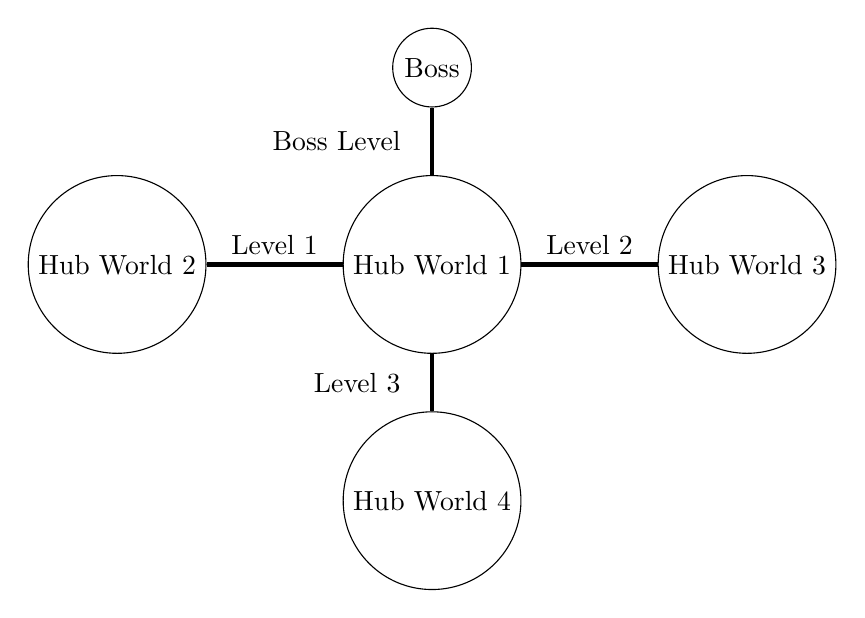
\begin{tikzpicture}
			\node[name=Hub-World-2,draw,circle,minimum size=1cm,inner sep=3pt] at (-4,0) {Hub World 2};
			\node[name=Hub-World-1,draw,circle,minimum size=1cm,inner sep=3pt] at (0,0) {Hub World 1};
			\node[name=Hub-World-3,draw,circle,minimum size=1cm,inner sep=3pt] at (4,0) {Hub World 3};
			\node[name=Hub-World-4,draw,circle,minimum size=1cm,inner sep=3pt] at (0,-3) {Hub World 4};
			\node[name=Boss,draw,circle,minimum size=1cm,inner sep=-1pt] at (0,2.5) {Boss};
			
			\path [draw] (Hub-World-2) -- node[name=Level-1, midway, above] {Level 1} (Hub-World-1);
			\path [draw] (Hub-World-1) -- node[name=Level-2, midway, above] {Level 2} (Hub-World-3);
			\path [draw] (Hub-World-1) -- node[name=Level-3, text width=3cm, midway] {Level 3} (Hub-World-4);
			\path [draw] (Hub-World-1) -- node[name=Boss-Level, text width=4.05cm, midway] {Boss Level} (Boss);
			
			\draw[ultra thick] (Hub-World-2) -- (Hub-World-1);
			\draw[ultra thick] (Hub-World-1) -- (Hub-World-3);
			\draw[ultra thick] (Hub-World-1) -- (Hub-World-4);
			\draw[ultra thick] (Hub-World-1) -- (Boss);
		\end{tikzpicture}
		%\caption{This displays the map for each World} \label{Map}
	\end{center}
	% if figure \newline \newline
	%\subsubsection*{Route 6}
	\textbf{Route 6} is the first World of \textbf{Title}. This is a man-made urban city built around a large metropolis arranged with roads and rails. In this World, not only will the player learns how to play the game, but will also buy parts to create a vehicle (i.e., motorcycle, car) used for a few levels that involve riding on highways. Brands include \textit{Autozone} and \textit{Advance Auto Parts}. It includes the levels Ivory Road, Cobalt Thruway, and Scarlet Bridge. The boss is \_ (see \nameref{MechaSally}) in the level Steel Convoy. \newline \newline
	%\subsubsection*{Candy Country}
	\textbf{Candy Country} is the second World of \textbf{Title}. This is a happy land filled with candies, chocolate, cake and castles. In this World, the player will buy tools to dig underground and various locations in the levels and find rare candies that can be sold at any Hub World in this World. Brands include \textit{Bed Bath \& Beyond}, \textit{Crate \& Barrel} and \textit{Pottery Barn}. It includes the levels Cake Desert, Chocolate Conduit, and Jelly Jubilee. The boss is \_ (see \nameref{MechaSally}) in the level Soda Springs. \newline \newline
	%\subsubsection*{Aqua Beach}
	\textbf{Aqua Beach} is the third World of \textbf{Title}. \iffalse This is an island-themed World that features \_. \fi In this World, the player will buy gear for riding on water. Brands include \textit{Quiksilver} and \textit{Billabong}. It includes the levels Coastal Shore, Fruity Jungle, and Tubular Aquarium. The boss is \_ (see \nameref{MechaSally}) in the level Cerulean Harbor. \newline \newline
	%\subsubsection*{Winter Paradise}
	\textbf{Winter Paradise} is the fourth World of \textbf{Title}. \iffalse This is an ice-based World that features \_. \fi In this World, the player will buy gear for staying warm and riding on ice. Brands include \textit{The North Face}, \textit{Columbia}, \textit{Timberland}, and \textit{Spyder}. It includes the levels Frosty Mountains, Snowy Village, and Polar Park. The boss is \_ (see \nameref{MechaSally}) in the level Chilly Casino. \newline \newline
	%\subsubsection*{Vernal Forest}
	\textbf{Vernal Forest} is the fifth World of \textbf{Title}. \iffalse This is a forest-themed World that features \_. \fi In this World, the player will buy gear for surviving the outdoors. Brands include \textit{L.L.Bean}, \textit{REI}, and \textit{Dick's Sporting Goods}. It includes the levels Dawn Hill, Dusk Woods, and Rainy Cave. The boss is \_ (see \nameref{MechaSally}) in the level Abandoned Castle. \newline \newline
	%\subsubsection*{Game Network}
	\textbf{Game Network} is the seventh World of \textbf{Title}. \iffalse This is a cyberspace-based World that features \_. \fi In this World, the player will buy unique gifts that will be used as tools for solving puzzles. Brands include \textit{Brookstone}, \textit{The Sharper Image}, and \textit{SkyMall}. It includes the levels Techno District, Time Rush, and Hidden Cyberpunk. The boss is \_ (see \nameref{MechaSally}) in the level Virus Void. \newline \newline
	%\subsection*{Astral Sky}
	\textbf{Astral Sky} is the eighth World of \textbf{Title}. This is a World high above the skies where ancient ruins and floating platforms are located. In this World, the player will buy mostly everything combined (from previous levels) including parts for a simple plane, gadgets, and wearable gear for flying through the skies. It includes the levels Star Realm, Cloud Highland, and Wish Garden. The boss is \_ (see \nameref{MechaSally}) in the level Serpent Jump. \newline \newline
	\textbf{TSX} is the ninth and final World of \textbf{Title}. It is basically the base located in outer space above the Earth. Here the player fights the final boss. That is \_ (see \nameref{MechaSally}).
	%\end{multicols}
	%includegraphics[width=in]{}
	\vfill
	\hrule
	\vspace{0.25cm} %\newline if \hrulefill
	[1] ``Hub World (Concept).'' \textit{Giant Bomb,} \href{www.giantbomb.com/hub-world/3015-1855/}{www.giantbomb.com/hub-world/3015-1855/}.
	\newpage
	\section*{GAME EXPERIENCE}
	After the Spadyal logo, the player is taken to the start screen. The player will have three options: New Game, Continue, Special, and Options. New Game lets the player begin to play the game for the first time. Continue takes the player to a menu where they saved their previous progress on the game. Special shows the player bonus materials and achievements (see \nameref{BonusMaterials} and \nameref{Achievements}); this option will only show if the player has beaten the game. Options lets players change the settings on the game. \newline \newline
	\noindent The beginning of the game will have a scene that lets the player play a short visual novel game---or ``interactive fiction that usually have very little in terms of gameplay but focus more on extensive storytelling, character interactions, dialogue trees, decision-making, and branching narratives, as well as artwork, cutscenes, voice acting, and music\textsuperscript{[2]}''---showing \_. After that little visual novel game, the gameplay begins.
	\begin{center}
		%\includegraphics[width=in]{GameExperience}
	\end{center}
	%\noindent The world and characters of \textbf{Title} \_ \newline \newline
	The music in \textbf{Title} should be electronic music---both melodic and heavy. It should be something different and interesting for the player to experience the rhythmic gameplay while listening to the music in the background.
	\vfill
	\hrule
	\vspace{0.25cm} %\newline if \hrulefill
	[2] ``Visual Novel.'' \textit{Giant Bomb,} \href{https://www.giantbomb.com/visual-novel/3015-2029/}{https://www.giantbomb.com/visual-novel/3015-2029/}.
	\newpage
	\section*{GAME MECHANICS}
	There are some of the hazards, equipment, gear, tools, clothing, and food available to the player.
	\subsection*{HAZARDS}
	
	\begin{multicols}{3}
		\begin{center}
			Ramming Cars \\
			Exploding Candy \\
			Slippery Ice \\\columnbreak
			Icicles \\
			Electrocuted Rollercoaster Rails \\
			Plant Platforms \\\columnbreak
			Spikes  \\
			Wormholes \\
			Thunderstorms
		\end{center}
	\end{multicols}
	\subsection*{EQUIPMENT/GEAR/TOOLS}
	Below are essential for the player to pass levels:
	\begin{itemize}[noitemsep]
		\item Car Parts
		\item Motorcycle Parts
		\item Spoons
		\item Summer (Water) Clothing
		\item Surf Gear
		\item Winter Clothing
		\item Winter Gear
		\item Spring (Outdoor) Clothing
		\item Outdoor Gear
		\item Electronic Gadgets
		\item Airplane Parts
		\item Rocket Parts
	\end{itemize}
	\subsection*{FOOD}
	Below might be useful for health and experience points as the player goes through each World:
	\begin{itemize}[noitemsep]
		\item Road Trip
		\begin{itemize}[noitemsep,nosep]
			\item Popcorn
			\item Chips
			\item Beef Jerky
			\item Water
		\end{itemize}
		\item Sweets
		\begin{itemize}[noitemsep,nosep]
			\item Cake
			\item Candy
			\item Chocolate
			\item Ice Cream
		\end{itemize}
		\item Summer
		\begin{itemize}[noitemsep,nosep]
			\item Ramune
			\item Cola
			\item Watermelon
			\item Iced Tea
		\end{itemize}
		\item Winter
		\begin{itemize}[noitemsep,nosep]
			\item Coffee
			\item Oatmeal
			\item Hot Chocolate
			\item Green Tea
		\end{itemize}
		\item Spring
		\begin{itemize}[noitemsep,nosep]
			\item Fruits
			\item Vegetables
			\item 
			\item 
		\end{itemize}
		\item Asian Food
		\begin{itemize}[noitemsep,nosep]
			\item Japanese Sushi
			\item Japanese Ramen
			\item Chinese Rice
			\item Chinese Egg Rolls
		\end{itemize}
	\end{itemize}
	\newpage
	\section*{ENEMIES}
	
	\section*{BOSSES}
	
	\begin{description}[align=right,labelwidth=3cm,noitemsep]
		\item [] \label{MechaSally}
		\item [] \label{MechaSally}
		\item [] \label{MechaSally}
		\item [] \label{MechaSally}
		\item [] \label{MechaSally}
		\item [] \label{MechaSally}
		\item [] \label{MechaSally}
		\item [] \label{MechaSally}
		\item [] \label{MechaSally}
	\end{description}
	\newpage
	\section*{BONUS MATERIALS} \label{BonusMaterials}
	If the player beats the entire game, the player will receive a digital copy of Title Vol. 1. This exciting 200 page light novel features \_ and illustrations.
	\section*{ACHIEVEMENTS} \label{Achievements}
	\begin{description}[align=right,labelwidth=3cm]
		\item [Money Saver] 
		\item [Man of Tesla] 
		\item [] 
		\item [] 
		\item [] 
		\item [] 
		\item [] 
		\item [] 
	\end{description}	
	\newpage
	\section*{MONETIZATION PLAN}
	Since this game is a free download (from the website), the player will be able to collect and spend one currency in the game: \textbf{Dollars (\$)}. %\textbf{Yen (\textyen)}.
	\begin{center}
		\textbf{\Huge \$}
	\end{center}
	\subsection*{Shops}
	Each Hub World has either a mall, plaza, or a small shopping center where the player can buy tools/equipment, gear, parts, and food. \newline \newline
	Each shop can let the player have a shopping cart gathering store items before paying. If the player were to walk out of the store, the items won't be removed from their shopping cart until $(5 < x < 10) \textrm{ where } x$ is the number of minutes in the range has passed; this will be called a ``Clipboard.'' \newline \newline
	*\textit{The player's history of purchases will be recorded in a database for an achievement.}
	\subsection*{Yen}
	At the beginning of the game, the player earns \$300 \iffalse 34,000 \$ ($\approx$ \$302) \fi. \$ can be found in the following types of stages:
	\begin{description}[align=right,labelwidth=3cm,noitemsep]
		\item [Fight Level:] \$ can be picked up after defeating an enemy, dropping \$ behind
		\item [Platform Level:] \$ can be picked up in several areas of this type of level, including shortcuts and secret areas
		\item [Dig Level:] \$ can be found in secret areas underground
		\item [Stealth Level:] \$ can be found in secret areas of a building, site, etc.
		\item [Combo Level:] all of the above
	\end{description}
	\section*{MARKETING PLAN}
	
	\vfill
	\begin{center}
		\textbf{\Huge Compiled with \LaTeX}
	\end{center}
\end{document}